
\chapter{Quantum Circuits}


\section{Introducing Tensor Products}

\begin{example}
Show that the tensor product distributes over vector addition.
\end{example}

This is a special case of the bilinearity property with 
the scalars set to 1 and $v' = 0$. 


\section{Matrix Tensor Products}

\begin{example}
An \textit{outer product} is an intersting case where normal \textit{matrix multiplication} 
gives the same operation the same as a tensor product. 
An \textit{outer product} is normal matrix multiplication of a column vector on the left multiplying 
a row vector on the right. \\
\textbf{(a)} Determine $(4,2,7)(1\; 2\; 6)$ and $(1,2,6) \otimes (4,2,7)$   \\ 
\textbf{(b)} Show that $v_1 v_2 = v_1 \otimes v_2$ for any two vectors in $\mathbb{C}^2$  \\ 
\textbf{(c)} Prove that $v_1 v_2 = v_1 \otimes v_2$ for general vectors.

\end{example}


\highlightdef{\textbf{Multiplication Property}: 
$(M \otimes N)(M' \otimes N') = (MM') \otimes (NN')$}

\frmrule

Using the Dirac bra-ket nototation, the previous result can 
be written as: $\ket{\psi_1}\bra{\psi_2} = \ket{\psi_1} \otimes \bra{\psi_2}$

\section{Composite Systems}


\highlightdef{$n = \text{number of qubits}$, $N = \text{number of basis vectors}$}

\begin{example}
For one system with state $\frac{1}{\sqrt{2}} \ket{0} + \frac{1}{\sqrt{2}} \ket{1}$
and second system with state $\frac{1}{\sqrt{2}} \ket{0} + \frac{\sqrt{3}}{2} \ket{1}$ 
find the state of the \textit{composite system}.
\end{example}

\frameans{}{
$
\frac{1}{2\sqrt{2}} \ket{00} + 
\frac{\sqrt{3}}{2\sqrt{2}} \ket{01} + 
\frac{1}{2\sqrt{2}} \ket{10} + 
\frac{\sqrt{3}}{2\sqrt{2}} \ket{11}
$ 
}

\frmrule

The fact that we combined together \textit{more than one} tensor product 
and use \textit{different levels of nesting} causes us to lose the 
top-level factorisation. 


\begin{example}
Prove that the following two-qubit system \textit{cannot be factorised}
into two qubits. 
$$\ket{\psi} = \frac{1}{\sqrt{2}} \ket{00} + \frac{1}{\sqrt{2}} \ket{11}$$
\end{example}

\frmrule

Assume there is a factorisation. We can therefore express it in the following form. 

\[ \begin{array}{lll}
\ket{\psi} = \frac{1}{\sqrt{2}} \ket{00} + \frac{1}{\sqrt{2}} \ket{11} 
& = & (\alpha_0 \ket{0} + \alpha_1 \ket{1})(\beta_0 \ket{0} + \beta_1 \ket{1}) \\
& = & \alpha_0 \beta_0 \ket{00} + 
\alpha_0 \beta_1 \ket{01} + 
\alpha_1 \beta_0 \ket{10} + 
\alpha_1 \beta_1 \ket{11} \\
\end{array}\] 

Comparing coefficients we have the following: \\
$\alpha_0 \beta_0 = \frac{1}{\sqrt{2}}$,
$\alpha_0 \beta_1 = 0$,
$\alpha_1 \beta_0 = 0$ and
$\alpha_1 \beta_1 = \frac{1}{\sqrt{2}}$.

If we multiply eqn1 and eqn4 we get $\alpha_0 \alpha_1 \beta_0 \beta_1 = \frac{1}{2}$.
If we multiply eqn2 and eqn3 we get $\alpha_0 \alpha_1 \beta_0 \beta_1 = 0$.
And yet, $0 \neq \frac{1}{2}$. We have a contradiction and so the system has no factorisation. 

\frmrule

\begin{example}
For a general two-qubit state, $\ket{\psi}$, define the terms: \\
\textbf{(a)} \textit{separable state}
\textbf{(b)} \textit{entangled state}
\end{example}

\frameans{}{
separable state: $\ket{\psi}$ can be written as $\ket{x}\ket{y}$ \\
entangled state: $\ket{\psi}$ \textit{cannot} written as such
}

Asking ourselves whether a state is entangled is as simple as algebraic 
exercise of proving whether or not the factorisation exists. 

\highlightdef{\textbf{Entangled State} cannot be written as a product state}

However entanglement has a much richer meaning when we take this 
the definition and apply it at the atomic level to discover important physical consequences. 
In particular the discussion of \textit{Principle of Locality} and \textit{Local Realism}.
In Quantum Computing \highlightdef{entanglement is not 
seen as a \textit{problem} but rather as a useful \textit{resource}}

Later we will look at \textit{Quantum Encryption} where one can find out if somebody is 
evesdropping on a transmission via entanglement. Classical channels \textit{cannot} do this.
This gives a much more reliable test over how secure the channel is. 

\section{Measurement Revisited}


\begin{example}
For three-qubit state, $\ket{\psi} = \frac{1}{\sqrt{3}}(\ket{001} + \ket{010} + \ket{100})$
the first qubit is measured. Write down the possible outcomes,
and whether they are separable or entangled.


\end{example}

\frameans{}{
separable state: \ket{\psi} can be written as \ket{x}\ket{y} \\
entangled state: \ket{\psi} \textit{cannot} written as such
}


\highlightdef{\textbf{General Measurement Principle}: $\sum^{k}_{j=1} M^{H}_{j} M_{j} = I$}






\section{Introducing Quantum Circuits}



\begin{figure}
  \centerline{
    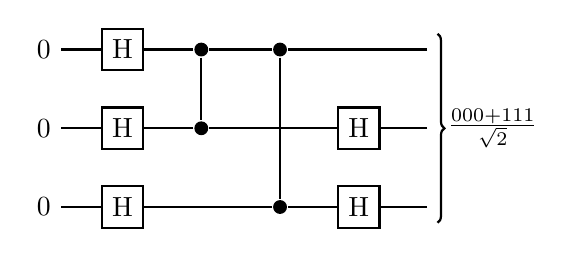
\begin{tikzpicture}[thick]
    %
    % `operator' will only be used by Hadamard (H) gates here.
    % `phase' is used for controlled phase gates (dots).
    \tikzstyle{operator} = [draw,fill=white,minimum size=1.5em] 
    \tikzstyle{phase} = [fill,shape=circle,minimum size=5pt,inner sep=0pt]
    \tikzstyle{surround} = [fill=black!10,drop shadow,draw=black]
    %
    % Qubits
    \node at (0,0) (q1) {\ket{0}};
    \node at (0,-1) (q2) {\ket{0}};
    \node at (0,-2) (q3) {\ket{0}};
    %
    % Column 1
    \node[operator] (op11) at (1,0) {H} edge [-] (q1);
    \node[operator] (op21) at (1,-1) {H} edge [-] (q2);
    \node[operator] (op31) at (1,-2) {H} edge [-] (q3);
    %
    % Column 3
    \node[phase] (phase11) at (2,0) {} edge [-] (op11);
    \node[phase] (phase12) at (2,-1) {} edge [-] (op21);
    \draw[-] (phase11) -- (phase12);
    %
    % Column 4
    \node[phase] (phase21) at (3,0) {} edge [-] (phase11);
    \node[phase] (phase23) at (3,-2) {} edge [-] (op31);
    \draw[-] (phase21) -- (phase23);
    %
    % Column 5
    \node[operator] (op24) at (4,-1) {H} edge [-] (phase12);
    \node[operator] (op34) at (4,-2) {H} edge [-] (phase23);
    %
    % Column 6
    \node (end1) at (5,0) {} edge [-] (phase21);
    \node (end2) at (5,-1) {} edge [-] (op24);
    \node (end3) at (5,-2) {} edge [-] (op34);
    %
    % Bracket
    \draw[decorate,decoration={brace},thick] (5,0.2) to
    node[midway,right] (bracket) {$\frac{\ket{000}+\ket{111}}{\sqrt{2}}$}
    (5,-2.2);
    \end{tikzpicture}
  }
  \caption{
    A quantum circuit for producing a GHZ state using
    Hadamard gates and controlled phase gates.
  }
\end{figure}



\section{Universal Sets}

Recall from Computational Techniques, 
the definition of the \textit{Euclidean Norm}.


\highlightdef{\textit{Every} unitary operator $U$, on the space $\mathbb{C}^{n}$
can be represented by a product of $C(n,2)$ \textit{two-level unitary matrices}}

Every unitary matrix has at most $C(n,2)$ degrees of freedom. 
This is how many elements are in upper triangle plus the diagonal. 
So the idea is to decompose the matrix into the product of 
$C(n,2)$ matrices where each degree of freedom turns into the multiplication of rank one matrix. 

\frmrule 

\begin{example}
Find a quantum circuit that uses single qubit transforms and CNOTs to implement the transform on three qubits.
$$
M = \begin{bmatrix}
       1 & 0 & 0 & 0 & 0 & 0 & 0 & 0  \\
       0 & 1 & 0 & 0 & 0 & 0 & 0 & 0  \\
       0 & 0 & a & 0 & 0 & 0 & 0 & c  \\
       0 & 0 & 0 & 1 & 0 & 0 & 0 & 0  \\
       0 & 0 & 0 & 0 & 1 & 0 & 0 & 0  \\
       0 & 0 & 0 & 0 & 0 & 1 & 0 & 0  \\
       0 & 0 & 0 & 0 & 0 & 0 & 1 & 0  \\
       0 & 0 & b & 0 & 0 & 0 & 0 & d  \\
     \end{bmatrix}
$$
\end{example}


\section{Reversible Computation}

\highlightdef{\textbf{Reversible Computation}: \textit{Every} quantum circuit is \textit{reversible}}




\section{Implementing Classical Circuits}

Is there a method for converting classical algorithms into quantum algorithms?
A classical algorithm or \textit{classical circuit} is $f : \{0,1\}^n \rightarrow \{0,1\}$
Thinking of classical algorithms as being simply a function is perfectly acceptable 
according to the \textit{Church-Turing Thesis}, a thesis which gives 
suggests that Turing machines form the definition 
for what an algorithm actually is.

Quantum computers attack the Church-Turing thesis (any algorithmic
process can be efficiently simulated using a Turing
machine).

\highlightdef{A quantum computer can implement mimic the possibly
\textit{several} classical steps for computing $f$ by using just \textit{one unitary operator} }

In principle, quantum computation is able to subsume classical computation.


\highlightdef{Classical circuits are, in general, \textit{irreversible}}. 
There are classical models of computation that can be reversed, but we will ignore them.



This is a consequence of the \textit{pidgeon-hole principle}. 
We have a surjective function that is not an injection. So 
there is no chance that $f$ is invertible. 
Although, NOT gate is an example of an invertible (reversible) gate,
there are many classical gates such as AND, XOR, NAND that are \textit{irreverisble} (non-invertible).

We \textit{can} implement classical circuits with quantum circuits, 
but quantum gates are always unitary and therefore reversible. 
The result is that we have \textit{ancilla bits} and \textit{garbage bits}. 
The ancilla and garbage are additional bits that are only important for 
making the computation reversible.


\begin{example}
A quantum circuit consisting of a \textit{controlled swap} can be used to 
implement the classical circuit consisting of an AND gate.

Suppose use inputs $a$, $b$ and 0. Here 0 is an \textit{ancilla bit}.
We want to know the outputs from this circuit. To do this, 
let's draw a truth table for all the possible input values.




Hence The outputs from the circuit are ..., ... and ........

\frameans{}{$a$, $\neg a \wedge b$ and $a \wedge b$  }

The third input qubit is an 
\textit{ancilla bit} and the second output bit 
is a \textit{garbage bit}.



\highlightdef{We want to remove $\ket{junk(x)}$ so that \textit{interference isn't prevented} }

We erase the junk (replace with zero), 
replace the output $f(x)$ with the input $x$ 
and add $y \oplus f(x)$.

There is no junk associated with the input, $\ket{junk(x)}$.
Instead with have $y \oplus f(x)$. Now interference isn't prevented.


\end{example}